\section{System Design}
\label{sec-design}
As mentioned above, we designed merging layers in our network so that we can process the input images by performing convolution operations to each single image, and then merging them together. The merged data will be stacked with the feature maps of each single image before we perform the next layer of convolution on them. Each convolutional layer uses the same set of parameters for all the images, so that the same set of features are extracted from the images, and thus can be merged. The merging layers consists of simple calculations extracting either the most significant, or the mutual features of the images, the former preserving interesting findings while the latter filters out credible features from the redundancy of the input. The network pipeline consists of alternate layers of convolution and merging, and after each merging layer, the reliable information accumulates and more complex features can be extracted with their support. Furthermore, we frequently insert the original input images in each level of our pipeline, creating an unevenness in depth and reducing network complexity, because we discovered that this process guides the model to be loyal to the inputs, generating more truthful results and less artifacts.

The details of our network architecture is as follows:
	Each input image (or each lane from the output of the previous layer) is assigned to its own lane and processed by several convolutional layers. These layers share parameters across channels; however, each image is processed individually and do not interact with each other in this stage. Each channel will present a feature map of n channels.
	The features extracted from all layers are merged broadwise with the following function:


    $${x'_k=\sum x_ie^{kx_i}/\sum e^{kx_i}}$$


Where k varies from -1 to 1. Apparently, k=0 leads to averaging, k=${+\infty}$ leads to a process similar to max operator and k=${-\infty}$ leads to min operator. This process merges information from every lane into one. The output is n channels for each value of k. 
	The original input images are accessed again. These images are also processed separately by several convolutional layers (sharing parameters across lanes) to extract features. The output of these images (m channels each) are stacked with the n channels from step 2) as m+n channels each lane. Some more convolution and an upscaling layer may follow, merging the data more thoroughly. These will be the input for the next layer.
The above 3 steps are stacked as one layer. The functional network often consists of 5 to 8 layers to achieve 4x super resolution. The network ends with a merging process similar to the 2) step and a few more layers of convolution. The full structure of a 3 layer network is shown in Fig~\ref{fig-system}.

\begin{figure}
 \centering
    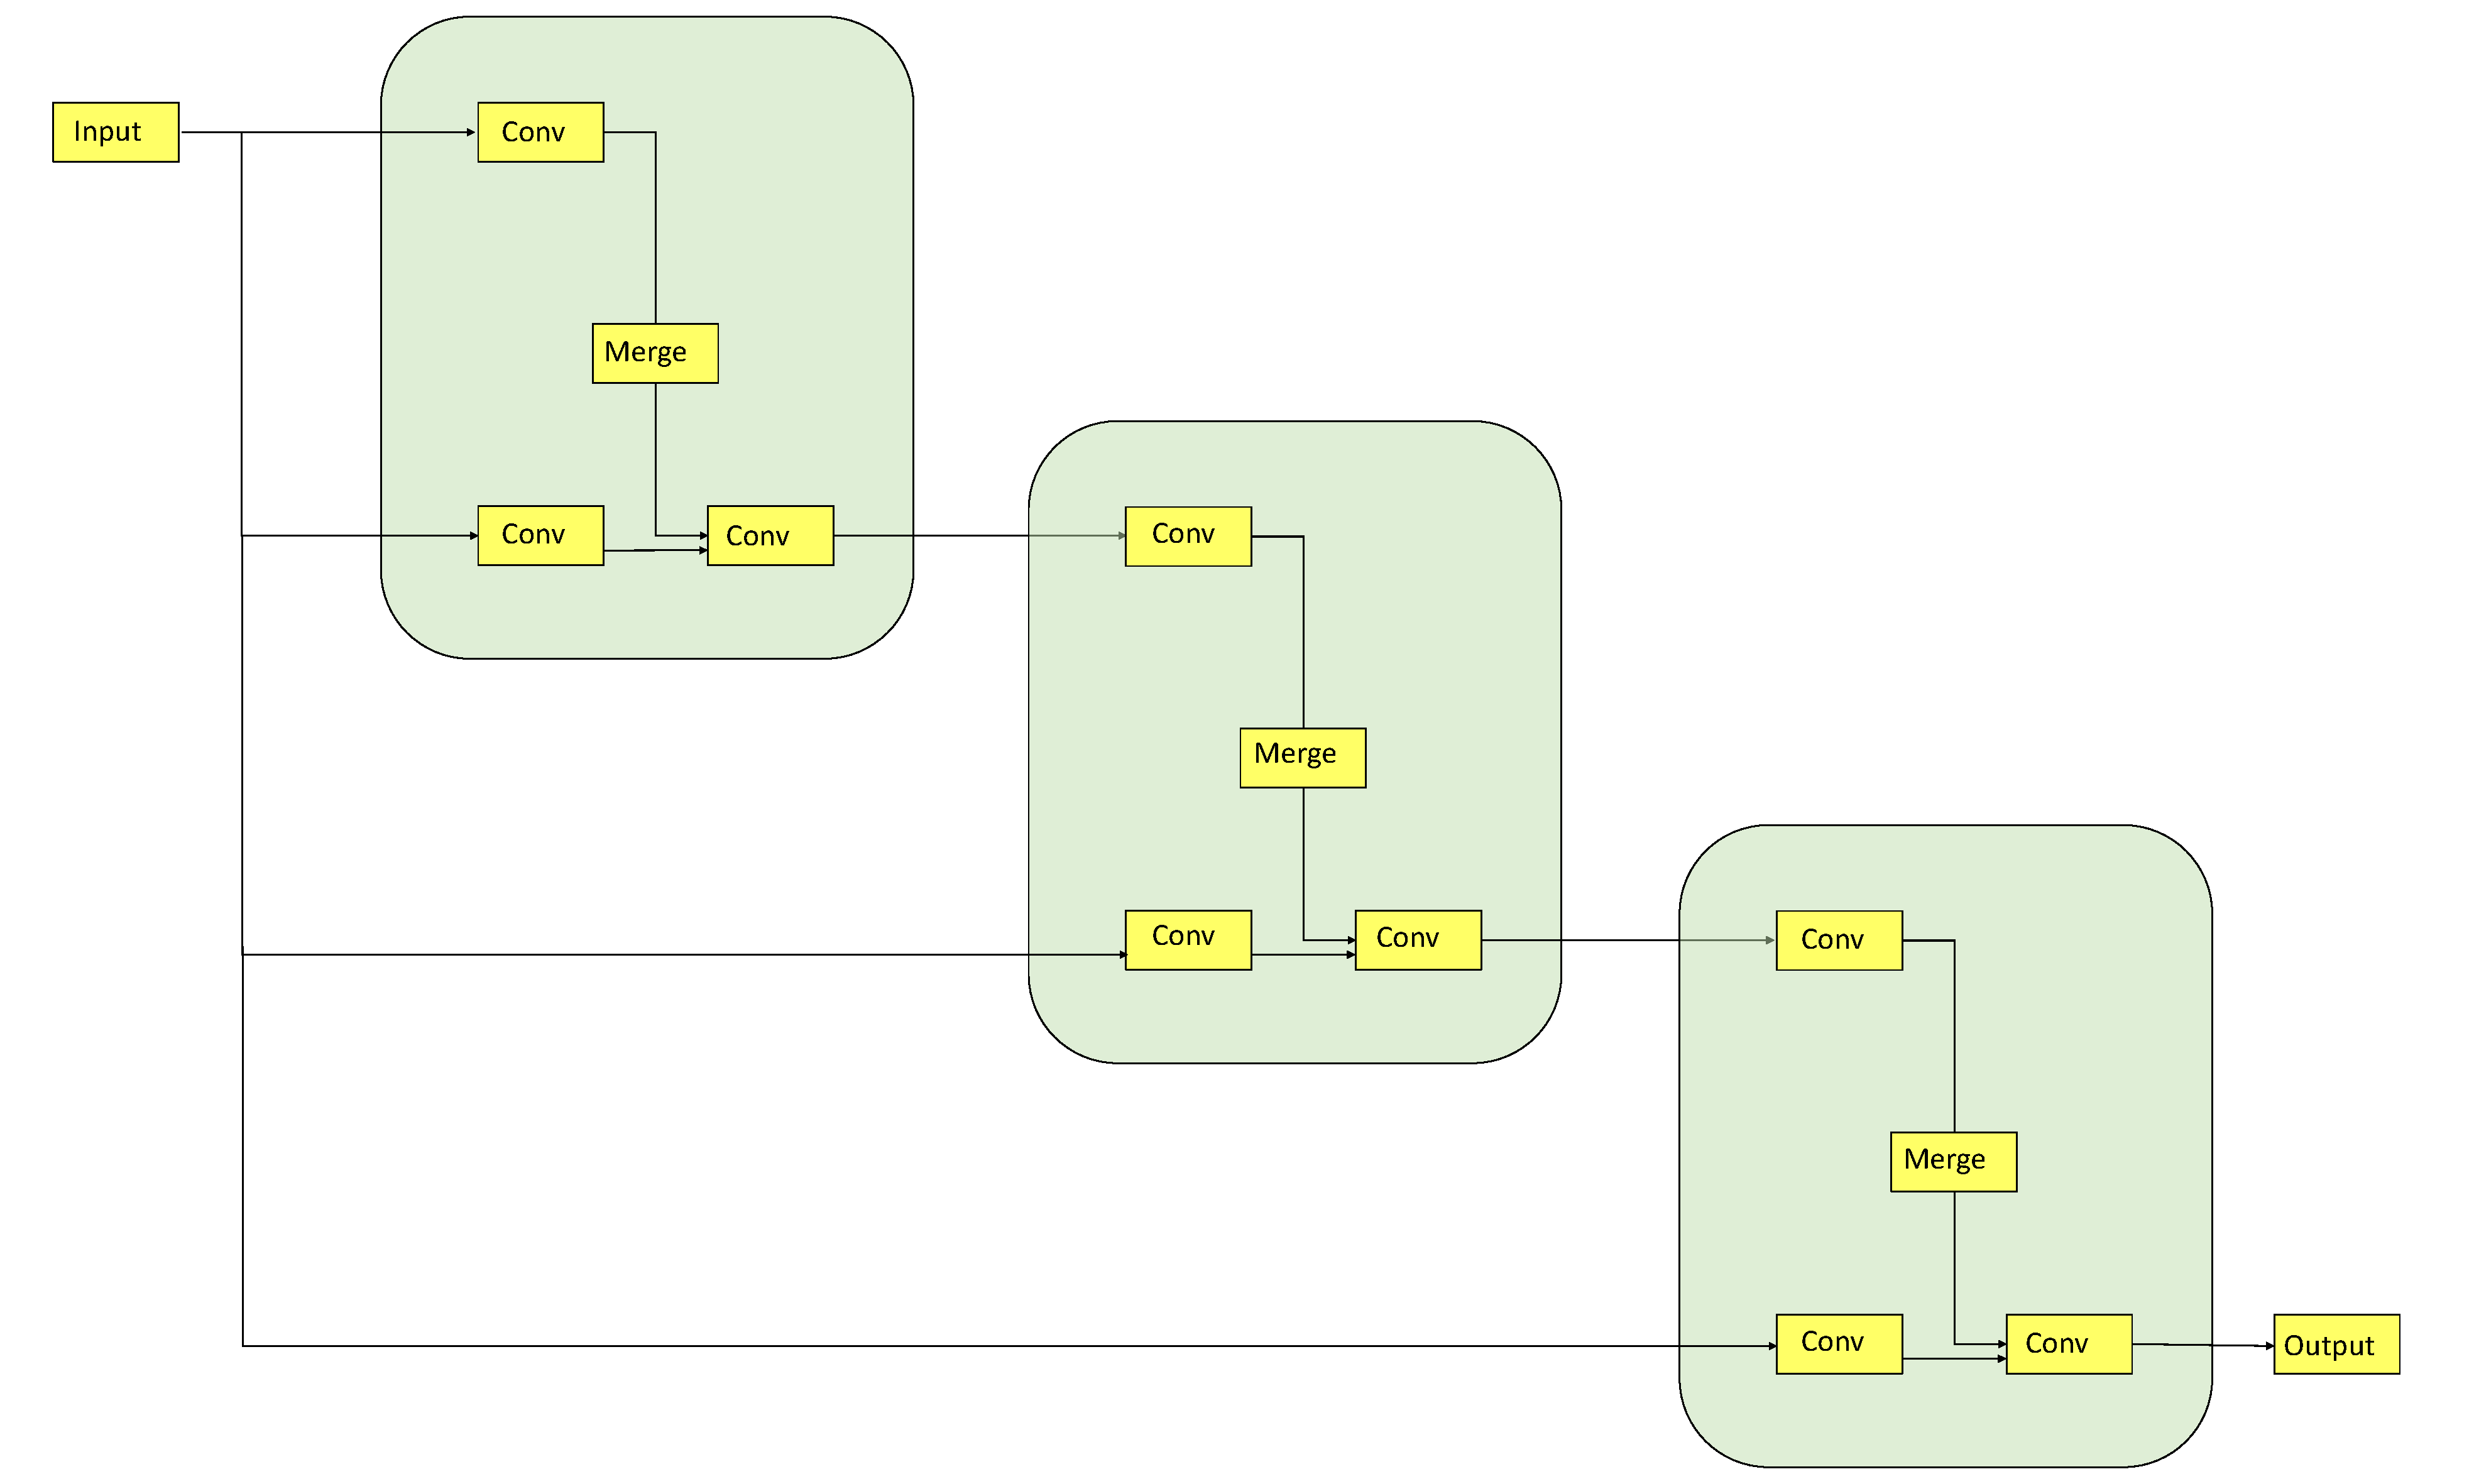
\includegraphics[width=0.5\textwidth]{./pic/design.pdf}
    \caption{Network Architecture of SRPeek.}
    \label{fig-system}
\end{figure}
